\documentclass[a4paper]{article}
\usepackage{amssymb}
\usepackage{bbm}
\usepackage[normalem]{ulem}
\usepackage{graphicx}
\usepackage[colorlinks,linkcolor=blue,anchorcolor=blue,citecolor=blue,urlcolor=blue]{hyperref}
\usepackage{mciteplus}
\usepackage{etoolbox}
\usepackage{subcaption}
\usepackage{tikz}
\usetikzlibrary{shapes}
\usepackage{fontspec}

\title{Statement of Research}
\author{JinGuo Liu\\ Department of Physics, Harvard University}
\date{\today}

\newcommand*\circled[1]{\tikz[baseline=(char.base)]{
            \node[shape=circle,draw,inner sep=1pt] (char) {#1};}}
\newcommand{\<}{\langle}
\renewcommand{\>}{\rangle}
\newcommand{\vsigma}{\vec{\sigma}}
\setlength{\topmargin}{-10mm}
\setlength{\textwidth}{7in}
\setlength{\oddsidemargin}{-8mm}
\setlength{\textheight}{9in}
\setlength{\footskip}{1in}

\newfontfamily\DejaSans{DejaVu Sans}

\begin{document}
\fontsize{10}{13}
\selectfont
\maketitle

I am a Post-Doctoral fellow in Mikhail Lukin's group at the department of physics at Harvard University with an interest in understanding the connection between computing and physics.
%In the past decades, these two seemingly unrelated fields are increasingly inter-weaved, bringing solid works that deepened our understanding about the nature of computation and the nature of our physical world.
%For example, by relating the energy dissipation in a computational process and an open quantum system, researchers showed why the Landauer's principle (every irreversible operation to a bit requires dissipating an energy lower bounded by $k_bT\ln 2$ to the environment) is correct from a pure quantum perspective~\cite{Reeb2014}; 
%by relating the dynamics of a local Hamiltonian with a universal quantum Turing machine, researchers showed the problem of telling whether a local Hamiltonian or an initial state can thermalize or not is uncomputable~\cite{Shiraishi2021}, i.e. as hard as the famous halting problem in computer science.
%How quantum computers can help to understand the hardness of a classical computational task.
The majority of my current research is about understanding the computational hardness and its relation to quantum physics, which I believe is the key to understanding the nature of computation.
In the following, I will explain my works in the past two years mainly from two aspects, one is understanding the computational hardness from the solution space properties, and another is embedding computational-hard problems in a physical system.

\section{Solution space properties of hard combinatorial optimization problems}
\subsection{Current Work}
In the past two years, I have been most dedicated to creating a unified framework to solve the \textit{solution space properties}~\cite{Liu2022} of a class of hard combinatorial optimization problems. Here, the solution space property refers to a class of quantities that not only include the maximum or minimum set size, but also include the number of sets at a given size, enumeration of all sets at a given size, and direct sampling of such sets when they are too large to be fit into memory; the class of problem includes but is not limited to the independent set problem, the maximum cut problem, the vertex coloring problem, the maximal clique problem, the dominating set problem, and the satisfiability problem, among others. The framework I and my collaborators created is called generic tensor network, where the word ``generic'' comes from generic programming in computer science.
While the relationship between a counting problem and a tensor network is well known, these works did not catch much attention of computational scientists due to their limited use cases.
We take a different view of a tensor network and show how different solution space properties can be computed with the same program by elevating the tensor element algebra to commutative semiring algebras.
% as show in Figure \ref{fig:venn-diagram}.
%which is highly inspired by the recent advances about random tensor network benchmarking quantum supremacy.
We show the real algebra is related to the counting of all solutions, the (extended) tropical algebra is related to the largest solution size(s), the polynomial algebra is related to the graph polynomials, the truncated polynomial algebra is related to the degeneracy of solutions with largest or smallest several sizes, the bit string algebra is related to finding one best solution, and the set algebra is related to solution enumeration.

% \begin{figure}[th]
%   \centering
% \centerline{\begin{tikzpicture}[]
%     \scriptsize
%     \node[draw,fill=lime!80,fill opacity=1, text opacity=1.0,ellipse,minimum width=2cm, minimum height=1cm,inner sep=0pt] at (0, 2.5) (R) {$\mathbbm{R}$};
%     \def\dx{-3};
%     \node[draw,fill=teal!50,fill opacity=1, text opacity=1.0,ellipse,minimum width=5cm, minimum height=3cm,inner sep=0pt] at (\dx, 0) (PN) {\hspace{-3.5cm}Polynomial};
%     \node[draw,fill=brown!75,fill opacity=1, text opacity=1.0,ellipse,minimum width=3.5cm, minimum height=1.0cm,inner sep=0pt] at (\dx, 0.7) (P1) {\hspace{-1.0cm}Largest order};
%     \node[draw,fill=brown!40,fill opacity=1, text opacity=1.0,ellipse,minimum width=3.5cm, minimum height=1.0cm,inner sep=0pt] at (\dx, -0.4) (P2) {\hspace{-0.8cm}Largest 2 orders};
%     \node[draw,fill=brown,fill opacity=1, text opacity=1.0,ellipse,minimum width=0.8cm, minimum height=0.3cm,inner sep=0pt] at (\dx, 1.0) (T) {};
%     \node[draw,fill=brown!50,fill opacity=1, text opacity=1.0,ellipse,minimum width=0.8cm, minimum height=0.3cm,inner sep=0pt] at (\dx, -0.1) (T2) {};
%     \node at (\dx, -1.2) {$\ldots$};
%     \node[above = 1cm] at (T) (textT) {Tropical};
%     \node[below = 2cm, left=4cm] (textT2) {Extended Tropical};
%     \draw[black,-latex] (textT) -- (T);
%     \draw[black,-latex] (textT2) -- (T2);

%     % set and set sampler
%     \node[draw,fill=yellow,fill opacity=0.5, text opacity=1.0,ellipse,minimum width=5cm, minimum height=3cm,inner sep=0pt] at (0, 0) (SN) {};
%     \node[below of=1] at (SN) {Set};
%     \node[draw,fill=red!70,fill opacity=0.5, text opacity=1.0,ellipse,minimum width=4cm, minimum height=1.5cm,inner sep=0pt] at (-0.5, 0) (S1) {\hspace{1.5cm}Bit string};
% \end{tikzpicture}}

%     \caption{The the tensor network element types used in this work and their relationships.
%     The overlap between two ellipses indicates that a new algebra can be created by combining those two algebras. ``Largest order'' and ``Largest 2 orders'' mean truncating the polynomial by only keeping its largest or largest two orders.} \label{fig:venn-diagram}
% \end{figure}


% benefit to open source community
I created an open-source package \href{https://github.com/QuEraComputing/GenericTensorNetworks.jl}{GenericTensorNetworks} (will be public on Github soon) that might benefit people in the field of computational complexity and statistic physics.
During the development of this package, I also contributed a lot to the open-source community. I and Chris Elrod wrote the package \href{https://github.com/TensorBFS/TropicalGEMM.jl/}{TropicalGEMM} for fast tropical matrix multiplication, which has a very close to the theoretical optimal speed, i.e. half the speed of floating-point number; I rewrote the tensor permutation in Julia base and CUDA to speed up the high-rank tensor manipulation; I wrote the package \href{https://github.com/TensorBFS/OMEinsumContractionOrders.jl}{OMEinsumContractionOrders} for the state of the art \texttt{einsum} contraction order optimization.

% the understanding we have

This project is highly motivated by another experimental project that I participated in, where we use variational quantum algorithms to solve the maximum independent set (MIS) problem on a diagonal-coupled unit-disk grid graph (DUGG) by embedding a problem instance into a Rydberg atom array Hamiltonian~\cite{Ebadi2022}.
In this experiment, it is crucially important to explain why our quantum algorithm works better than classical simulated annealing in some graph instances but not in others.
The results found by using the generic tensor network deepened our understanding of the MIS experiment.
By checking the degeneracies of independent set solutions at different sizes, we find that the degeneracy ratio can be a good indicator of the classical hardness of a problem instance.
By inspecting the configuration space connectivity, we find the absence of the overlap-gap-properties~\cite{Gamarnik2021} in most of the target problems.
Here, the overlap gap property is an important feature of a solution space geometry, the presence of which indicates a no-go for a local-search-based algorithm.
These solution space properties that helped understand quantum and classical algorithms are not feasible in the previous frameworks that mainly targeted on best solutions. Our method fills the gap between finding one solution for a hard problem and understanding a hard problem.

\subsection{Future Work}

It would like to generalize the idea of generic programming to other algorithms using the inclusion-exclusion principle or subset convolution and see what new properties can be computed.
To this end, it is worth mentioning dynamic programming.
Dynamic programming is closely related to a tropical tensor network, for example, the Viterbi algorithm for finding the most probable configuration in a hidden Markov model can be interpreted as a matrix product state featured with tropical algebra, and the tropical tensor network in the main text is probably equivalent to dynamic programming in finding the best solution.
However, while having broader applications,
dynamic programming does not have a clear algebraic interpretation required by computing solution space properties beyond finding the best solution.

\section{Solving the maximum independent set problem with Rydberg atom arrays}
\subsection{Current Work}
I and my collaborators proposed a scheme to reduce the MIS problem on a general graph to one on a DUGG and showed this reduction is very likely to be optimal~\cite{Liu2022b}.
The proposed method only introduce an overhead that is linear to the pathwidth of the source graph, where the pathwidth is a graph characteristic that is upper bounded by the number of vertices.
This result may have impacts on both fields of quantum computing and computational complexity.

In the quantum computing field, it is a crucial step toward solving the MIS problem on a general graph with quantum algorithms implemented on Rydberg atom arrays that have highly constrained two-dimensional geometry.
In the previous MIS experiment paper, we studied the MIS problem on a DUGG. We showed although DUGGs have highly constrained topology, finding their MISs is nevertheless NP-complete.
However the reduction in that paper from an MIS problem on a general graph to an MIS problem on DUGG has an overhead of $n^8$.
If one wants to solve an MIS problem on a general graph with $100$ vertices, which can be solved in a classical computer in milliseconds, the required number of qubits is $\sim10^{16}$, which is a number not feasible in the near term.
Our new mapping scheme resolved these concerns.

In the computational complexity field, it can bridge some important results about the MIS problem. For example, a lemma of our reduction is: the MIS size of a unit-disk graph is hard to approximate with an error smaller than $\sqrt{n}$ because the MIS size of a general graph is hard to approximate within $n^{1-\epsilon}$~\cite{Hastad1996}.

% Reducing one hard problem to another is a widely used technique to prove the computational hardness of a certain problem.
% While this new reduction is not the first work showing the NP-completeness of the MIS problem on DUGG~\cite{Ebadi2022}, why do we think it is important (we are patenting it as an important application in Rydberg atom arrays) to quantum algorithms and computational complexity study?
% The fact is, although we showed how to map a general MIS problem to one on DUGG in our experiment paper, that reduction has an overhead of $O(n^8)$.
%Most algorithms implementable on Rydberg atom arrays have a fundamental constraint of the two dimensional layout of the optical traps.
%Then it is crucially important to reduce a more general NP-hard problem, e.g. the MIS problem on a general graph, to the MIS problem on a unit-disk graph. Where a unit-disk graph is a graph that embedded in a two dimensional Euclidean space such that two vertices are connected if an only if they are separated by a distance small than a threshold value $r_0$.
%In the MIS experiment paper, we studied the MIS problem on a DUGG.
%Although DUGGs have highly constraint topology, finding a maximum independent sets of which is nevertheless NP-complete.
%This imply the existence of a polynomial time reduction from this problem to other NP-complete problems, however, the previously best known algorithm to map a general maximum independent set problem to an independent set problem on DUGG has an overhead of $n^8$.
%If one wants to solve an MIS problem on a general graph with $100$ vertices, which can be solved in a classical computer in milliseconds, the required number of qubits is $\sim10^{16}$, which is a number not feasible in near term.
%The new reduction scheme I and my collaborators proposed changes the game because it only introduces an overhead that proportional to pathwidth of a graph, where the pathwidth of a graph is a graph characteristic that upper bounded by the number of vertices, i.e. the number of vertices in the mapped graph is at most $O(n^2)$.
%Most interestingly, we also show this mapping is very likely to be optimal.
%This result can bridge some important results in field of computational complexity, e.g. the MIS size of a unit-disk graph is hard to approximate within $n^{0.5}$ because the MIS size of a general graph is hard to approximate within $n^{1-\epsilon}$~\cite{Hastad1996}.
% For sparse graphs like tree graphs and three regular graphs, this quantity can be much smaller than the number of vertices.
The paper for this work as well as an open source software will be released soon.

\section{Future Work}

%DUGGs have many properties that make them look simple, like the absence of overlap gap property in a random instance, the treewidth that scales square root of the size, and can be constant-approximated in polynomial time, unlike the general MIS problem.
%We also have a preliminary simulated annealing result that indicates an average DUGG can be solved in polynomial time, which is too good to be true.
%One possible explanation is: the mapped graphs live in the hardest corner of the whole set of DUGGs.
%I want to study and understand DUGGs more to explain these observations seemingly inconsistent with our previous understanding.
%I also want to study the quantum dynamics of the mapped graph under annealing and deepen my understanding of the performance of quantum annealing on this may be the hardest portion of DUGGs.

\subsection{New computational frameworks}
One of the most important goals of quantum physics is building new computational frameworks that can be much better than traditional CMOS based technologies.
I think reducing the energy consumption and making use of quantum entanglement might be the most important two directions to go.
Since there are a lot researchers already understand the importance of quantum computing.
I want to put more efforts to reducing the energy consumption. Although it is widely accepted that quantum computing is a type of reversible computing, a quantum computer is often built in a energy in-efficient style.
For example, if one wants to apply a quantum gate with precision $\epsilon$, the energy consumption might be $1/\epsilon$.
I haven't estimated the energy consumption of realizing the Shor's algorithm upto the desired precision to crack the encryption system.
But I think it might be much, and I will do it in the future.
After all, the energy consumption is the crucial measure of computing efficiency rather than the computing time.




In traditional reversible computing, most proposed frameworks are the von-Neuman architecture that requires a RAM.
Then except the reversible logic gates, they also need to design a protocal to access the memory reversiblly.
To me, developing a reversible RAM and let the data transport through the BUS reversibly is not very practical.
Another type of physics like computing based on block cellular automata does not have such problem.
There might be $10^6$ room known to optimize comparing to the brain of a honeybee.

\subsubsection{Reversible Cellular Automata on Rydberg atom arrays}
I propose implementing quantum cellular automata in Rydberg atom arrays as a practical approach towards universal quantum computing for the following reasons
\begin{enumerate}
    \item Cellular automata does not require local pulses, which is costly in Rydberg atom arrays,
    \item Cellular automata does not require runtime atom moving, which is costly in Rydberg atom arrays,
    \item Cellular automata can be parallelized easily.
\end{enumerate}

To build a block quantum cellular automata (BQCM), \circled{1} we first prepare two piles of Rydberg atoms in hyper-fine states $|0\rangle$ and $|1\rangle$.
\circled{2} Then initialize the configuration by moving atoms to a bi-layer square lattice. We map two atoms at the same $x,y$-coordinate to a qudit, and each qudit has 4 possible states $|00\rangle = 0$, $|01\rangle=1$, $|10\rangle=\square$ and $|11\rangle=\blacksquare$.
We use these qudits to encodes both the program and the input data.
\circled{3} Divide the square lattice into A, B sub-lattices as shown in Fig.~\ref{fig:ablattice} and drive them to do circular moves of period $T$, with the phases of A, B sub-lattices different by $\pi$. Each time four atoms move closest to each other, perform a gate operation that does the quantum gate in Fig.~\ref{fig:basicgate}. After certain steps $m$, the results can be read from the final configuration.

\begin{figure}[th]
  \centering
  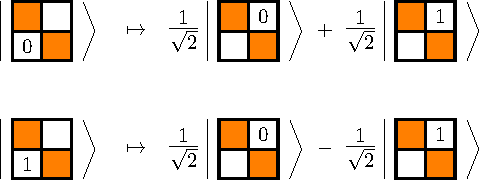
\includegraphics[width=\columnwidth]{images/bqca-hadamard.pdf}
\end{figure}

\begin{figure}[th]
  \centering
  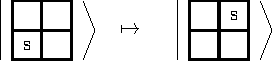
\includegraphics[width=\columnwidth]{images/bqca-signal.pdf}
\end{figure}

\begin{figure}[th]
  \centering
  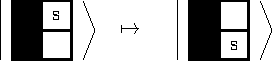
\includegraphics[width=\columnwidth]{images/bqca-bouncing.pdf}
\end{figure}

\begin{figure}[th]
  \centering
  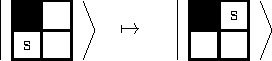
\includegraphics[width=\columnwidth]{images/bqca-signal1.pdf}
\end{figure}

\begin{figure}[th]
  \centering
  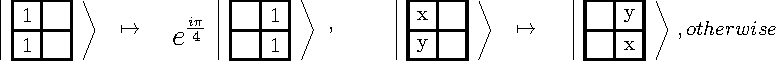
\includegraphics[width=\columnwidth]{images/bqca-cphase.pdf}
\end{figure}

NOTE: initial configurations can be $\{0, 1, r, {\rm no~atom}\}$
\subsection{Characterizing the solution space of hard problems}


\section{Summary}
To summarize, at this point in my career, my primary interests are computational-hard problems and near-term quantum algorithms.
In the future, I want to understand the nature of computational hardness more from the aspects of quantum thermal dynamics and the integrability of a quantum system.
Except for these research interests, I want to devote half of my time to the help build up the open-source scientific software ecosystem.
I believe programming is a proper way to formalize some part of human knowledge, and open-source software development is an integrable and collaborative practice in this direction.
% way for human to build up the tree of knowledge.
%If there is only one thing I can do in my life, I wish I can grow this tree a bit; given the fact that we are living in a world that open source software developers are never fairly paid, I desperately need a faculty position {\DejaSans ☺}. %, for example, Julia is the best candidate at the moment.
\bibliographystyle{unsrt}
\bibliography{ref}
\end{document}
